\documentclass{tufte-book}

\hypersetup{colorlinks}% uncomment this line if you prefer colored hyperlinks (e.g., for onscreen viewing)

%%
% Book metadata
\title{B547 Assignment 1}
%\author[The Tufte-LaTeX Developers]{The Tufte-LaTeX\ Developers}
\author[Pat Shaffer Akshada More DongInn Kim John Stein]{Pat Shaffer Akshada More DongInn Kim John Stein}
\publisher{Indiana University\smallcaps{   submitted: Feb 10, 2017}}

%%
% If they're installed, use Bergamo and Chantilly from www.fontsite.com.
% They're clones of Bembo and Gill Sans, respectively.
%\IfFileExists{bergamo.sty}{\usepackage[osf]{bergamo}}{}% Bembo
%\IfFileExists{chantill.sty}{\usepackage{chantill}}{}% Gill Sans

%\usepackage{microtype}


%%
% For nicely typeset tabular material
\usepackage{booktabs}

\usepackage{lscape}
% \usepackage{rotating}
\usepackage[figuresright]{rotating}
%%
% For graphics / images
\usepackage{graphicx}
\setkeys{Gin}{width=\linewidth,totalheight=\textheight,keepaspectratio}
\graphicspath{{graphics/}}

% The fancyvrb package lets us customize the formatting of verbatim
% environments.  We use a slightly smaller font.
\usepackage{fancyvrb}
\fvset{fontsize=\normalsize}

%%
% Prints argument within hanging parentheses (i.e., parentheses that take
% up no horizontal space).  Useful in tabular environments.
\newcommand{\hangp}[1]{\makebox[0pt][r]{(}#1\makebox[0pt][l]{)}}

%%
% Prints an asterisk that takes up no horizontal space.
% Useful in tabular environments.
\newcommand{\hangstar}{\makebox[0pt][l]{*}}

%%
% Prints a trailing space in a smart way.
\usepackage{xspace}


% Prints the month name (e.g., January) and the year (e.g., 2008)
\newcommand{\monthyear}{%
  \ifcase\month\or January\or February\or March\or April\or May\or June\or
  July\or August\or September\or October\or November\or
  December\fi\space\number\year
}

%adds a page number to each page
\fancypagestyle{plain}{}

% allows landscape environment
\usepackage{lscape}

% Prints an epigraph and speaker in sans serif, all-caps type.
\newcommand{\openepigraph}[2]{%
  %\sffamily\fontsize{14}{16}\selectfont
  \begin{fullwidth}
  \sffamily\large
  \begin{doublespace}
  \noindent\allcaps{#1}\\% epigraph
  \noindent\allcaps{#2}% author
  \end{doublespace}
  \end{fullwidth}
}

% Inserts a blank page
\newcommand{\blankpage}{\newpage\hbox{}\thispagestyle{empty}\newpage}

% Add trademark symbol
\usepackage{textcomp}

% Fixme Package
\usepackage[draft,footnote,nomargin]{fixme}

% allow drafting and editing functions
\usepackage[draft]{changes}
\newcommand{\mustfix}[1]{\fixme{\hl{#1}}}
\newcommand{\pleasenote}[1]{\fxnote{\hl{#1}}}
\newcommand{\john}[1]{{\textcolor{blue}{John: #1}}}
\newcommand{\akshada}[1]{{\textcolor{green}{Akshada: #1}}}
\newcommand{\donginn}[1]{{\textcolor{purple}{DongInn: #1}}}
\newcommand{\pat}[1]{{\textcolor{red}{Pat: #1}}}
\newcommand{\del}[1]{{\textcolor{gray}{#1}}}

\usepackage{units}

% Typesets the font size, leading, and measure in the form of 10/12x26 pc.
\newcommand{\measure}[3]{#1/#2$\times$\unit[#3]{pc}}

% Macros for typesetting the documentation
\newcommand{\hlred}[1]{\textcolor{Maroon}{#1}}% prints in red
\newcommand{\hangleft}[1]{\makebox[0pt][r]{#1}}
\newcommand{\hairsp}{\hspace{1pt}}% hair space
\newcommand{\hquad}{\hskip0.5em\relax}% half quad space
\newcommand{\TODO}{\textcolor{red}{\bf TODO!}\xspace}
\newcommand{\ie}{\textit{i.\hairsp{}e.}\xspace}
\newcommand{\eg}{\textit{e.\hairsp{}g.}\xspace}
\newcommand{\na}{\quad--}% used in tables for N/A cells
\providecommand{\XeLaTeX}{X\lower.5ex\hbox{\kern-0.15em\reflectbox{E}}\kern-0.1em\LaTeX}
\newcommand{\tXeLaTeX}{\XeLaTeX\index{XeLaTeX@\protect\XeLaTeX}}
% \index{\texttt{\textbackslash xyz}@\hangleft{\texttt{\textbackslash}}\texttt{xyz}}
\newcommand{\tuftebs}{\symbol{'134}}% a backslash in tt type in OT1/T1
\newcommand{\doccmdnoindex}[2][]{\texttt{\tuftebs#2}}% command name -- adds backslash automatically (and doesn't add cmd to the index)
\newcommand{\doccmddef}[2][]{%
  \hlred{\texttt{\tuftebs#2}}\label{cmd:#2}%
  \ifthenelse{\isempty{#1}}%
    {% add the command to the index
      \index{#2 command@\protect\hangleft{\texttt{\tuftebs}}\texttt{#2}}% command name
    }%
    {% add the command and package to the index
      \index{#2 command@\protect\hangleft{\texttt{\tuftebs}}\texttt{#2} (\texttt{#1} package)}% command name
      \index{#1 package@\texttt{#1} package}\index{packages!#1@\texttt{#1}}% package name
    }%
}% command name -- adds backslash automatically
\newcommand{\doccmd}[2][]{%
  \texttt{\tuftebs#2}%
  \ifthenelse{\isempty{#1}}%
    {% add the command to the index
      \index{#2 command@\protect\hangleft{\texttt{\tuftebs}}\texttt{#2}}% command name
    }%
    {% add the command and package to the index
      \index{#2 command@\protect\hangleft{\texttt{\tuftebs}}\texttt{#2} (\texttt{#1} package)}% command name
      \index{#1 package@\texttt{#1} package}\index{packages!#1@\texttt{#1}}% package name
    }%
}% command name -- adds backslash automatically
\newcommand{\docopt}[1]{\ensuremath{\langle}\textrm{\textit{#1}}\ensuremath{\rangle}}% optional command argument
\newcommand{\docarg}[1]{\textrm{\textit{#1}}}% (required) command argument
\newenvironment{docspec}{\begin{quotation}\ttfamily\parskip0pt\parindent0pt\ignorespaces}{\end{quotation}}% command specification environment
\newcommand{\docenv}[1]{\texttt{#1}\index{#1 environment@\texttt{#1} environment}\index{environments!#1@\texttt{#1}}}% environment name
\newcommand{\docenvdef}[1]{\hlred{\texttt{#1}}\label{env:#1}\index{#1 environment@\texttt{#1} environment}\index{environments!#1@\texttt{#1}}}% environment name
\newcommand{\docpkg}[1]{\texttt{#1}\index{#1 package@\texttt{#1} package}\index{packages!#1@\texttt{#1}}}% package name
\newcommand{\doccls}[1]{\texttt{#1}}% document class name
\newcommand{\docclsopt}[1]{\texttt{#1}\index{#1 class option@\texttt{#1} class option}\index{class options!#1@\texttt{#1}}}% document class option name
\newcommand{\docclsoptdef}[1]{\hlred{\texttt{#1}}\label{clsopt:#1}\index{#1 class option@\texttt{#1} class option}\index{class options!#1@\texttt{#1}}}% document class option name defined
\newcommand{\docmsg}[2]{\bigskip\begin{fullwidth}\noindent\ttfamily#1\end{fullwidth}\medskip\par\noindent#2}
\newcommand{\docfilehook}[2]{\texttt{#1}\index{file hooks!#2}\index{#1@\texttt{#1}}}
\newcommand{\doccounter}[1]{\texttt{#1}\index{#1 counter@\texttt{#1} counter}}

\usepackage{enumitem}
\setlistdepth{9}

% Generates the index
\usepackage{makeidx}
\makeindex

\begin{document}
% r.3 full title page
\maketitle

% v.2 epigraphs
\newpage\thispagestyle{empty}
\openepigraph{%
I think computer viruses should count as life.  I think it says something about
human nature that the only form of life we have created so far is purely
destructive.  We've created life in our own image.
}{Stephen Hawking%, {\itshape Design, Form, and Chaos}
}
\vfill
\openepigraph{%
Companies spend millions of dollars on firewalls, encryption and secure access
devices, and it's money wasted, because none of these measures address the
weakest link in the security chain.
}{Kevin Mitnick}
\vfill
\openepigraph{%
Passwords are like underwear: you don't let people see it, you should change it
very often, and you shouldn't share it with strangers.
}{Chris Pirillo}
\vfill
\openepigraph{%
Building secure systems is hard.
}{Steve Myers}







% r.5 contents
\cleardoublepage
\tableofcontents

%\cleardoublepage
%\listoffigures

%\cleardoublepage
%\listoftables


% r.9 introduction
\cleardoublepage
\chapter*{Introduction}

This report satisfies the requirements of assignment 1\cite{2017myersa1handout}, which requires us to perform a \textit{comprehensive} threat model a password manager.  We are allowed discretion in the choice of architectures but the architecture should provide for the remembering of many passwords for websites, products, appliances and other uses which require passwords.
\par The report is limited to no more than 7 pages of diagrams and 40 pages total length.  The final product is a threat model of the system and any other documentation that would be necessary to understand how the proposed system would run.  If any sections of the threat model are empty, they should still be included in the report and the report should indicate
that they were intentionally left empty.

%%
% Start the main matter (normal chapters)
\mainmatter


\cleardoublepage
\chapter{System Overview}
\label{ch:System Overview}
The system modeled is a web-enabled password manager that resides on a
tamper resistant USB thumb drive, modeled after the
IronKey\texttrademark~secure USB thumb drive. The password manager
allows for a user to enjoy the benefits of a secure offline password
manager with the option of receiving software and firmware updates from the
cloud. The USB device also hosts an embedded crypto system which can be
leveraged to provide powerful cryptographic tools which provide some assurance
that the tools have not been compromised. Because security is the primary objective, the password file (the file which stores user names, passwords, and their associated applications, appliances, or domains) is not written to persistent media outside the USB device.

\begin{marginfigure}%
\centering
  
\includegraphics[width=0.25\linewidth]{s1000-vertical}
  \caption{Picture of the IronKey USB drive.  More information can be
found at \url{www.ironkey.com}}
  \label{fig:ik}
\end{marginfigure}



\section{System Description}
\label{sec:sysdesc}

The concept of operation is for the user to, after having inserted the device into a computer, launch the provided trusted application from the USB device, which has been mounted as a CD-ROM.  The application's public key is sent to the computer along with the application executable, and used to establish a temporary encrypted session with the USB (in which the corresponding private key is stored).  Within the temporary session, a random shared key is generated by the USB device and passed to the application to establish the secure application session.  Once the application is running, the user is in a secure but anonymous session with the USB device.  From this point, the user can choose to (a) submit a master password to the application in order to access his/her password store, (b) perform a secure software update on the device, or (c) perform a hard reset of the device, restoring the device to factory condition and losing any password store data.
\begin{enumerate}
    \item When the user submits his/her master password, the USB device will attempt to decrypt a header file stored on the device.  If successful, the device will initiate a secure user session with the application, encrypted using a the symmetric secure application key as well as a key derived from the user's password.  In this session, the user (via the application) may perform privileged operations with the password store file.
    \item When the user performs a secure software update, the application interrogates the web server as to the latest software release and downloads the digitally signed file.  Next, the application sends the file to the USB device for the update.  Within the USB device, the updated software is checked using the factory's public key and, if authentic, generates a new public/private key pair to store on the device, overwriting the current version of the software.  Finally, the USB device forces a restart of the device and the application using the new version.
    \item When the user elects to perform a hard reset on the device, the device overwrites the header file and password store file with a stored from-factory version, thereby permanently erasing any previously stored user password information and restoring the device to a factory state.
\end{enumerate}
\par The USB device firmware and software can be updated via a secure Internet
channel which accesses a webserver to download the device files to the USB
device.  Following download, the device authenticates the downloaded files and
updates the device.
The way to save the password via the password manager is straightforward. The
password is passed along with the corresponding key (e.g. a website, a username,
hostname, \dots) to the password manager when the secure user session is
setup as shown in Figures~\ref{fig:dfd_app} and ~\ref{fig:dfd_usb}. The key
must be unique. Once
the password is stored with the corresponding key to the encrypted partition in
the USB, a user can retrieve the password with the unique given key during the
secure user session. The retrieved password can be blinded out and copied to the
temporary memory of the system (e.g. clipboard) for users' convenience. Of
course, if a user inquires, the password can be displayed in a plain text but
preferably in an image format.

\begin{figure}
    \centering
    \includegraphics{DFD_Main}
    \caption{Main System Data Flow Diagram}
    \label{fig:dfd_main}
\end{figure}
\begin{figure*}
    \centering
    \includegraphics[width=\linewidth]{DFD_App}
    \caption{System Data Flow Diagram in the App side}
    \label{fig:dfd_app}
\end{figure*}

\begin{figure*}
    \centering
    \includegraphics[width=\linewidth]{DFD_USB}
    \caption{System Data Flow Diagram in the USB side}
    \label{fig:dfd_usb}
\end{figure*}

%\begin{figure*}
%    \centering
%    \includegraphics[width=0.8\linewidth]{webservdfd1}
%    \caption{System Data Flow Diagram for the Webserver}
%    \label{fig:wsdfd1}
%\end{figure*}


\begin{figure*}
    \centering
    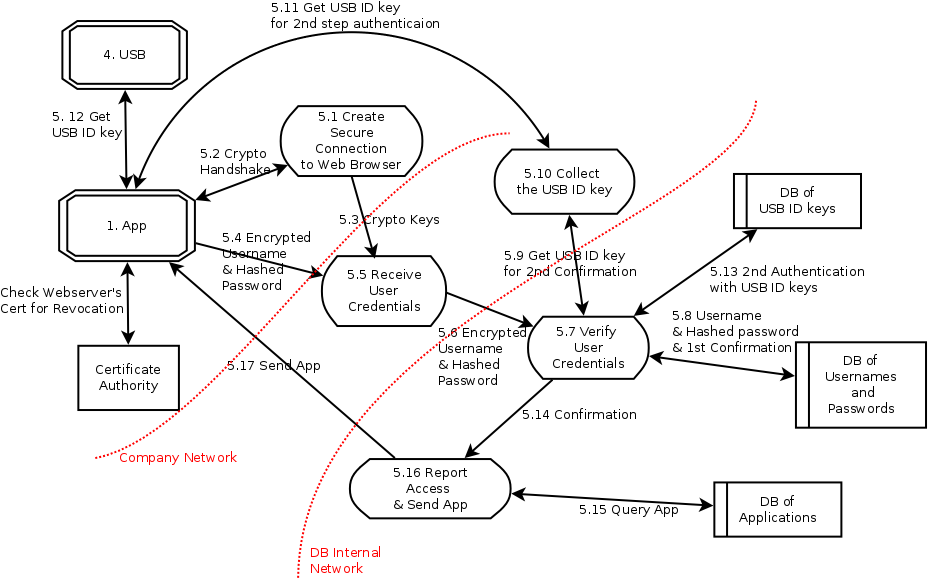
\includegraphics[width=0.8\linewidth]{DFD_Webserver}
    \caption{System Data Flow Diagram for the Webserverer}
    \label{fig:wsdfd}
\end{figure*}

The Password manager consists of two major components, the USB device and a User
Application. The USB device when plugged in the system is loaded as a CD
ROM. The Get/Load function from the application gets the public key and begins
the message
encryption. Once the user application is authenticated and loaded there can be 4
possibilities:
\begin{enumerate}
\item The password manager is used for the first time by the user
\item Correct credentials are entered by the user
\item Incorrect credentials are entered by the user
\item User enters incorrect credentials multiple times
\end{enumerate}

When the user uses the iron key for the first time, the header is decrypted with
the default key. Once the header decrypt is successful the user is forced to
reset the default password. When correct credentials are entered by the user,
the password key is sent to the USB which then decrypts the header with that
key.  Once the header is decrypted a a user session is started. The counter
which stores the number of invalid attempts is reset.The user has the option to
update the user password. The decrypted file is read into the memory and a new
password key and password file/header is written to the USB.A pair of key and
password is stored in the USB device. The password is queried from the USB
device using the given key.

If the user enters an invalid credentials, the header decrypt fails and the
password try counter is incremented.\marginnote{The USB itself does not possess
any logging capability save for the try counter which also serves as an
initiator to clear the system after a number of incorrect tries.} The user is
then prompted to enter a correct password. When a user enters a wrong password
multiple times which is equal to some threshold value, the reset counter
overwrites the header and password file by default.

The user application can be updated. When the update is successful, the USB is
updated and a force restart happens with the new version.When an update fails
the current version of the app is maintained.

The system data flow diagram is shown in figure \ref{fig:dfd_main}.


\section{Functional Requirements}
\label{sec:funcreq}
The functional requirements of the system are as follows:
\begin{enumerate}
    \item{Physically protect the USB against known tamper attacks including
physical attacks and USB electrical channel attacks.}\sidenote{We do not
enumerate all the possible USB physical and electrical attacks, nor do we
describe in detail the mitigations to these attacks.  It is assumed that
appropriate hardware antitamper features are incorporated into the USB design.}
    \item{Host all cryptography on the USB device.}
    \item{Allow for remote updates of USB software and firmware.}
    \item{Initiate device wipe after a set number of incorrect login attempts.}
    \item{Allow for the secure storage and retrieval of user websites and login
information.}
    \item{Provide for a secure, random password generator capability.}
\end{enumerate}


\cleardoublepage
\chapter{Threat Model}
\label{ch:threatmodel}
This chapter is the meat of the assignment.  We take the


\section{Adversary}
\label{sec:adversary}

\section{Assumptions}
\label{sec:assumptions}

\section{Threats}
\label{sec:threats}
In this section we identify the threat to each major element of our system, usually by using a dataflow diagram.  Use the subsections to enumerate and systematically walk through the threats.
\subsection{Threat Trees}
We conduct an analysis of each threat using a threat tree.

\subsection{STRIDE Modeling}
We conduct a STRIDE analysis on each major data flow or component.  The style does not allow for subsections so we may need to be a little creative and just use para


\cleardoublepage
\chapter{Mitigations}
\label{ch:mitigations}
In this chapter we describe the mitigations to the threats we found in
the previous chapter.

\section{Mitigation by Threat}

\section{Risk and Prioritization}
\label{sec:risk}
While it is beyond the scope of this assignment to describe any technical or
business processes used to manage risk, we implicitly manage risk through our
assumptions and mitigations.  For example, the risk from the threat of loss of
the USB (resulting in a denial of service) is transferred to the owner of the
device by assuming that the owner will take adequate precautions to prevent loss
or theft of the device.  For the unlikely lucky guess threat, the risk is
accepted because the likelihood of properly guessing a complex password in a
very small, fixed number of tries is unlikely.

\begin{marginfigure}
    \centering
    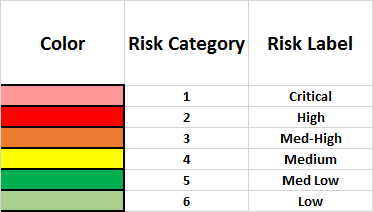
\includegraphics[width=\linewidth]{riskcats}
    \caption{Risk Categories Used in Threat Modeling}
    \label{fig:riskcats}
\end{marginfigure}

In general, we would expect to pay most attention to priority risks in
increasing order; for example, a category one risk would be addressed before a
category 3 threat risk.

\subsection{Risk Determination}
We used a modified OWASP risk methodology to determine the risks posed by each
threat or group of similar threats. Detailed information concerning the assessed
risks can be found in appendix 4.;


\cleardoublepage
\chapter{Conclusion}
\label{ch:conclusion}
The proposed system is a standalone password manager equipped with the
USB device. The device is hard to be tampered and is securely to store
the pair (e.g., key:password) of user's credentials, where the key is
a unique identity requiring to match the corresponding password
(e.g. website, hostname, username, \dots). The application of the USB
device provides an interface for a user to access the encrypted
partition in the USB device.  The credentials that a user wants to
store are located in the encrypted partition of the USB device which
can be decrypted only with the primary password that a user setup.
The default password is provided for the user to decrypt the encrypted
partition for the first usage. The application forces a user to update
the default password with a different password.  The USB device is
updated with the new release of the application which can be
downloaded from the designated webserver. The webserver uses the two
factor authentication to ensure the authentictiy and integrity of the
applications and the USB device. The user is required to register to
the website with the public key of the USB device.  The new
application is digitally signed with the factory's public key. Once
the new application is verified to be authentic, it replaces the
existing version in the USB device and restarts the application to
load up with the new version.

We have setup a threat model for the proposed system by using the
standard STRIDE threat.  Our threat model is based on the iterative
design. We review our proposed system architecture, dataflows, and
external entities. Any potential threats are identified by using the
STRIDE methodology and augmented by experimenting with the elevation
of privilege game cards.  We discuss any identified trheats and assign
a bug number to each one. Finally we decide whether we accept it as a
system risk or not and perfom a risk likelihood vs impact for all
accepted risks using a modified OWASP risk methodology.  We found 43
threats and identified 19 risks associated with the system threats. 10
high risks which are in the 2nd cartegory show that our proposed
system have relatively more high risks once it is compromised as shown
in Figure~\ref{fig:riskmatrix}. On the other hand, the likelihood of
the threats is 4.05 in average within 1 to 10 range and the 10 high
risks has 4.56. We have setup the attack tree with the scenario of
having the application of the device compromised while it is updated
as described in \nameref{ch:a4}. The risk of this threat is also high,
cartegory 2. It turns out that the proposed system is not vulnerable
in general and threats occur unlikely. However, if it is exploited,
the risks would be high.



\cleardoublepage
\chapter{Appendix 1: Security Exceptions and Assumptions}
\label{ch:a1}


This appendix contains tables describing the security assumptions used in the threat model.

\begin{table*}[h]
    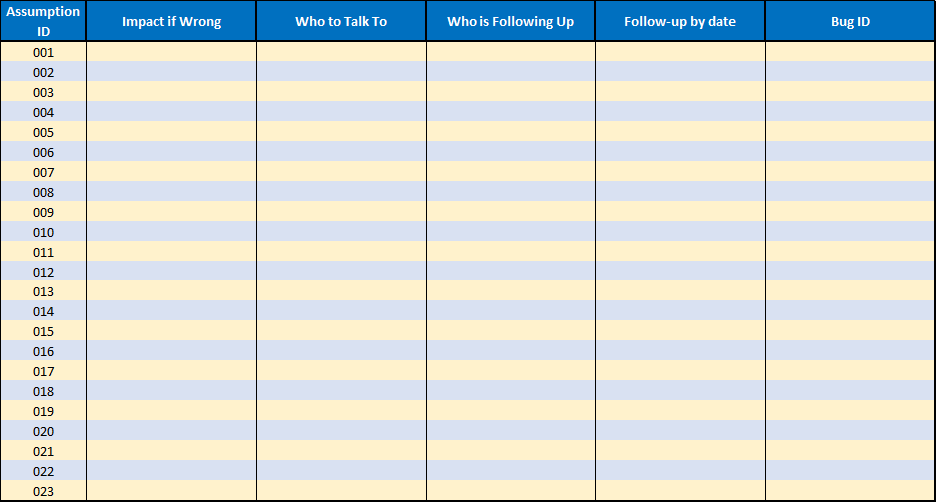
\includegraphics[width=\linewidth]{assumption_table_2017-02-03_14-13-43}
    \caption{Security Assumptions and Exceptions Table}
    \label{tab:sec_assumpt}
\end{table*}

\vfill



\cleardoublepage
\cleardoublepage
\chapter{Appendix 2: Threat List}
\label{ch:threatlist}

The final system threat table is shown in figure~\ref{tab:threatlist}.  Each
entry in the threat table has an associated ID, who found the threat, the DFD
diagram element which applies to the threat, the type of threat as given by the
STRIDE model, and a mitigation.  Each entry is also assign a bug ID and finally
a determination of whether the entry is accepted into the larger threat risk
table.  \marginnote{In practice, the use of design rules can be very effective
because they form tangible requirements which are push down to the lowest level
and then reviewed as the software product matures at each design review.  This
keeps key security practices up front and visible throughout the design process.
Finally,incorporating design rules into an evaluation plan ensures the integrety
and security of the final product.}
\par If one threat is similar to another, it may not be entered into the threat
table but rather a threat risk that best decstibes the collective threat is
entered into the table.  This does not mean that the threat is ignored as it
still has a bug id associated with it which must be dispositioned.  In some
cases the threat is not carried to the risk table but instead may be referred to
a design rule which is then checked off during software component design reviews
and testing.


\begin{table*}
\centering
  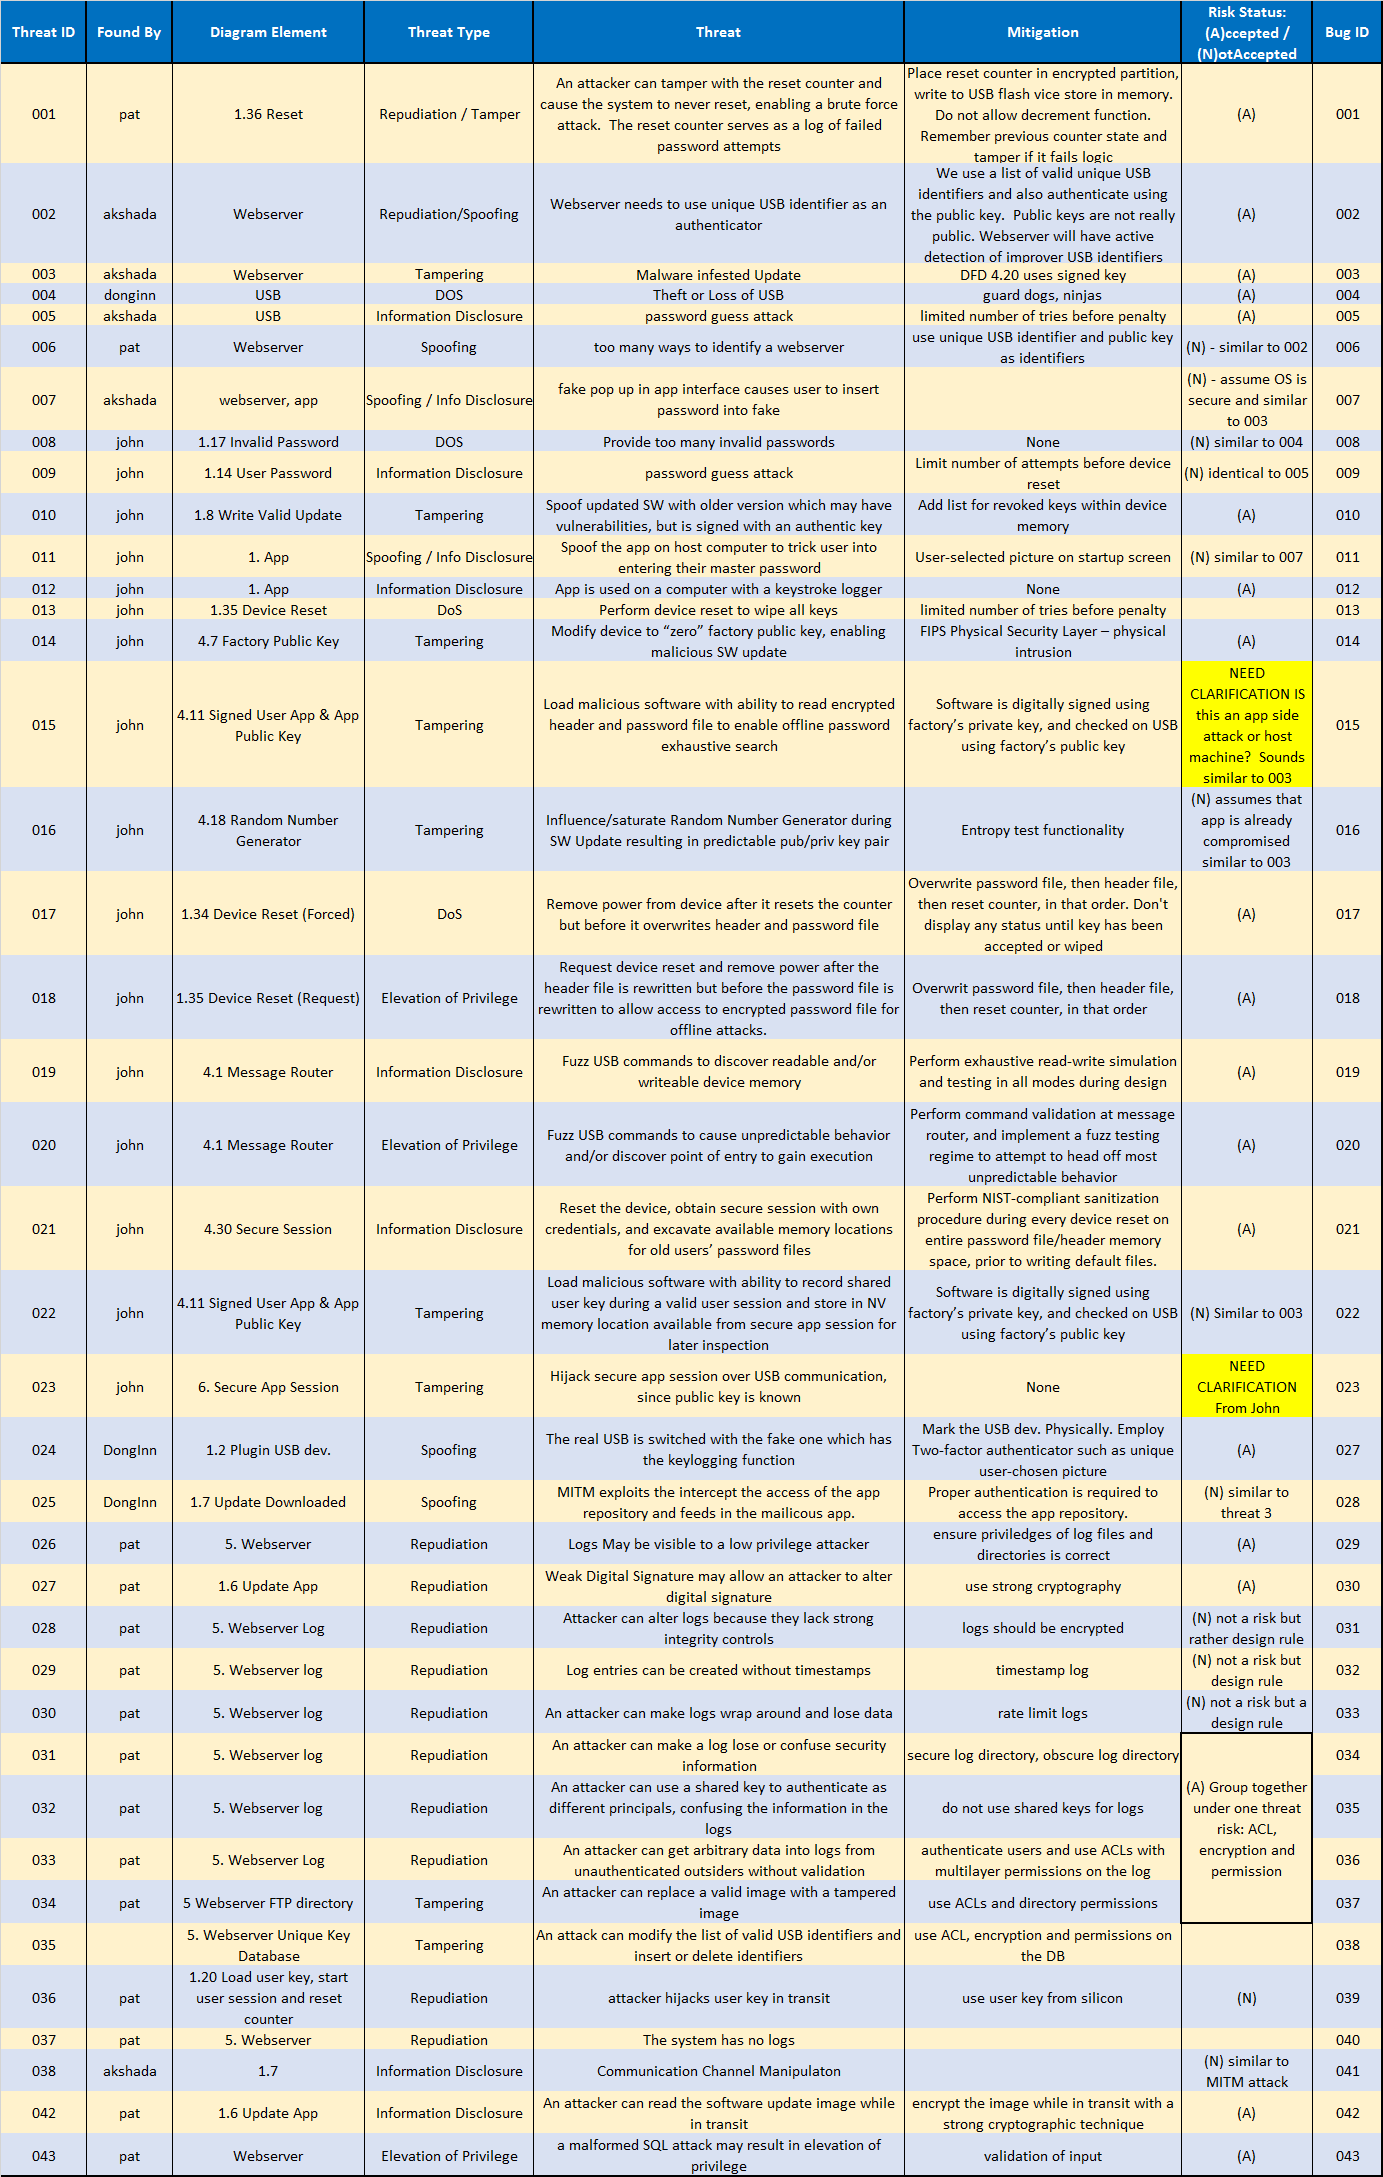
\includegraphics[width=\linewidth]{threat_list_final}
  \caption{Final Table of Threats}
  \label{tab:threatlist}
\end{table*}


%\cleardoublepage
%\chapter{Appendix 3: Mitigation List}
%\label{ch:a3}
%


\cleardoublepage
\chapter{Appendix 3: Risk Management Definitions and Methodology}
\label{ch:a3}

The risk methodology used in this assignment is taken from the OWASP Risk
Methodology~\cite{owasprisk} with modifications to the risk
matrix.\sidenote[][4.5cm]{OWASP uses a 3x3 table whereas we use a 5x5 table for
better granularity.}





Risk categories are defined in table ~\ref{tab:risk_cat}.\\


Each accepted threat is given a likelihood score which is based on threat agent
and vulnerability factors as well as an impact score which is based on technical
impact and business impact.  These two scores are used to enter the risk matrix
in figure~\ref{fig:riskmatrix} which will yield a risk category.

\begin{table}[h]
    \centering
    \begin{tabular}{l l l }
    \hline
    Risk Category & Definition \\
    \hline
    1 & Critical\\
    2 & High\\
    3 & Med-High\\
    4 & Med\\
    5 & Med-Low\\
    6 & Low \\
    \end{tabular}
    \caption{Risk Category Definitions}
    \label{tab:risk_cat}
\end{table}

\begin{table*}[ht]
    \centering
    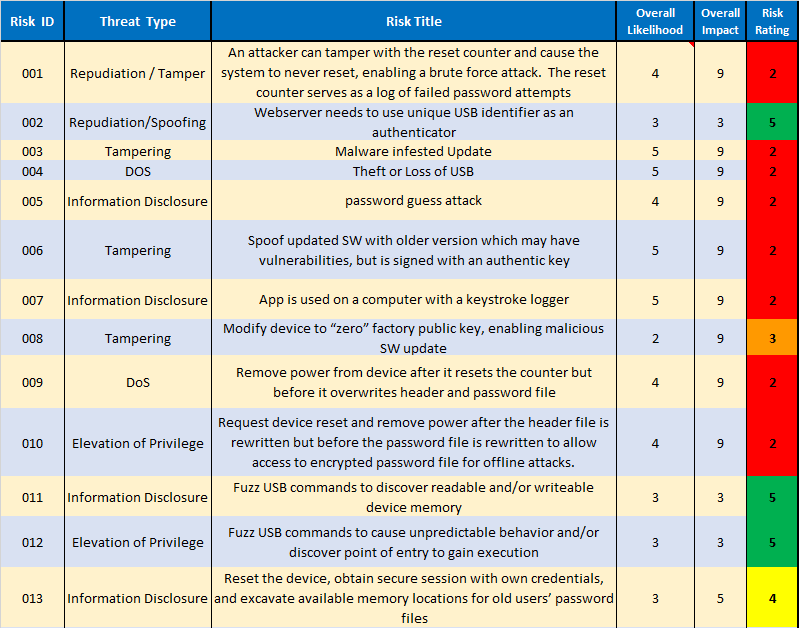
\includegraphics[width=\linewidth]{risk_sum}
    \caption{Threat Risk Summary Table}
    \label{tab:risksum}
\end{table*}


\begin{figure*}[]
    \centering
    \includegraphics[width=\linewidth]{risk_matrix}
    \caption{Populated Risk Matrix}
    \label{fig:riskmatrix}
\end{figure*}

By convention, category 1 or 2 risks require immediate attention and management
while category 5 and 6 risks can most likely be monitored.The password manager's
risk are summarized using the table in table~\ref{tab:risksum}.  Detailed
information concerning the factors used to asses likelihood and impact for each
risk is found in table~\ref{tab:likelihood} and table~\ref{tab:impact}.



\begin{sidewaystable}[]
    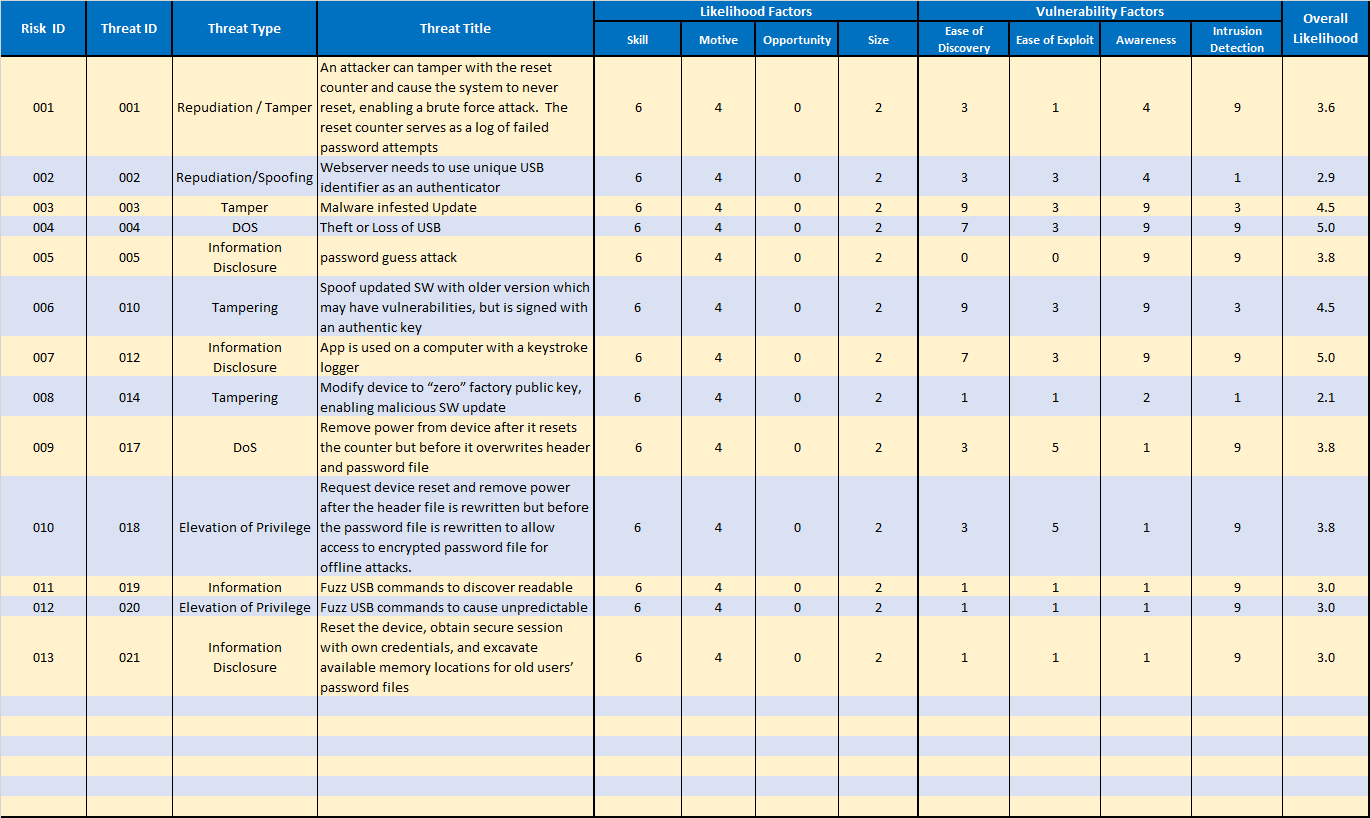
\includegraphics[]{owasp_likelihood}
    \caption{Threat Likelihood Table}
    \label{tab:likelihood}
\end{sidewaystable}


\begin{sidewaystable*}[]
    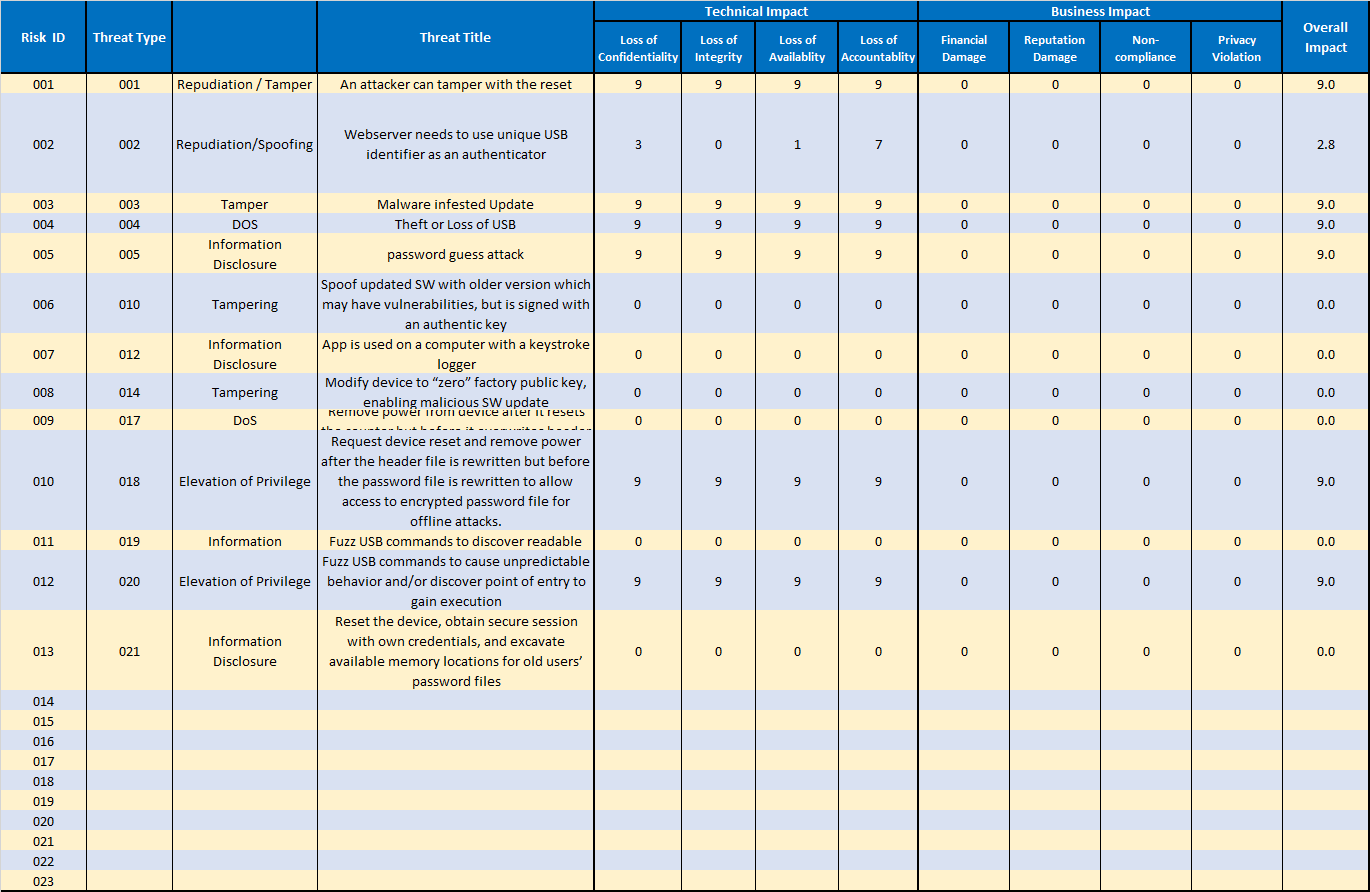
\includegraphics[]{owasp_impact}
    \caption{Threat Impact Table}
    \label{tab:impact}
\end{sidewaystable*}


\cleardoublepage
\chapter{Appendix 4: Attack Tree for Webserver Hosting Software/Firmware Updates}
\label{ch:a4}
\section{Attack Tree}
\newlist{myEnumerate}{enumerate}{9}
\setlist[myEnumerate,1]{label*=\arabic*.}
\setlist[myEnumerate,2]{label*=\arabic*.}
\setlist[myEnumerate,3]{label*=\arabic*.}
\setlist[myEnumerate,4]{label*=\arabic*.}
\setlist[myEnumerate,5]{label*=\arabic*.}
\setlist[myEnumerate,6]{label*=\arabic*.}
\setlist[myEnumerate,7]{label*=\arabic*.}
\setlist[myEnumerate,8]{label*=\arabic*.}
\setlist[myEnumerate,9]{label*=\arabic*.}

\begin{myEnumerate}

\item Compromise the software/firmware update
  \begin{myEnumerate}[label*=\arabic*.]
  \item Gather knowledge (and)
    \begin{myEnumerate}[label*=\arabic*.]
    \item Find the IP address or URL of the webserver (or)
      \begin{myEnumerate}[label*=\arabic*.]
      \item Google the website of the target USB
      \item Collect the static contents of the web site (e.g. CSS, javascript,
        images, \dots).
      \end{myEnumerate}
    \item Get the same model as the target USB
      \begin{myEnumerate}[label*=\arabic*.]
      \item Try to see if it is easy to feed in any malware/keylogger
      \end{myEnumerate}
    \item Find the place (IP range) where he/she uses the target USB
      \begin{myEnumerate}[label*=\arabic*.]
      \item Use port scanner in the same subnet
      \item Tap his/her network cable
      \item Find the public key of the target USB
      \end{myEnumerate}
    \end{myEnumerate}
  \item Build a fake web site which looks like the real one (and)
    \begin{myEnumerate}[label*=\arabic*.]
    \item Prepare the MITM attack
      \begin{myEnumerate}[label*=\arabic*.]
      \item Do the reverse engineering to build a malicious app to feed into the
        target USB
      \end{myEnumerate}
    \end{myEnumerate}
  \item Gain an access (and)
    \begin{myEnumerate}[label*=\arabic*.]
    \item Use the DNS Spoofing trick to redirect the victims access of app
      update to the fake website
      \begin{myEnumerate}[label*=\arabic*.]
      \item Wait until the target USB tries to access the website to get it updated (or)
        \begin{myEnumerate}[label*=\arabic*.]
        \item Intercept the connection to the real website (or)
          \begin{myEnumerate}[label*=\arabic*.]
          \item Push the malicious app/firmware (and)
            \begin{myEnumerate}[label*=\arabic*.]
            \item Collect all the passwords of the target USB
            \end{myEnumerate}
          \end{myEnumerate}
        \end{myEnumerate}
      \item Mail a fake notification of the new release of the app with the URL of
        the fake website
        \begin{myEnumerate}[label*=\arabic*.]
        \item Intercept the connection to the real website (or)
          \begin{myEnumerate}[label*=\arabic*.]
          \item Push the malicious app/firmware (and)
            \begin{myEnumerate}[label*=\arabic*.]
            \item Collect all the passwords of the target USB
            \end{myEnumerate}
          \end{myEnumerate}
        \end{myEnumerate}
      \end{myEnumerate}
    \item Use the IP Spoofing trick to intercept the victims access of app
      update to the fake website
      \begin{myEnumerate}[label*=\arabic*.]
      \item Wait until the target USB tries to access the website to get it updated (or)
        \begin{myEnumerate}[label*=\arabic*.]
        \item Intercept the connection to the real website (or)
          \begin{myEnumerate}[label*=\arabic*.]
          \item Push the malicious app/firmware (and)
            \begin{myEnumerate}[label*=\arabic*.]
            \item Collect all the passwords of the target USB
            \end{myEnumerate}
          \end{myEnumerate}
        \end{myEnumerate}
      \item Mail a fake notification of the new release of the app with the URL of
        the fake website
        \begin{myEnumerate}[label*=\arabic*.]
        \item Intercept the connection to the real website (or)
          \begin{myEnumerate}[label*=\arabic*.]
          \item Push the malicious app/firmware (and)
            \begin{myEnumerate}[label*=\arabic*.]
            \item Collect all the passwords of the target USB
            \end{myEnumerate}
          \end{myEnumerate}
        \end{myEnumerate}
      \end{myEnumerate}
    \end{myEnumerate}
  \end{myEnumerate}
\end{myEnumerate}




\bibliography{bibliography}
\bibliographystyle{plainnat}

\end{document}
